\section{Úvod}

Orientace v dějinách je často komplikovaná, zejména pokud se snažíme pochopit souvislosti mezi různými historickými událostmi, osobnostmi a směry. Setkáváme se s velkým objemem historických informací, letopočtů, významných událostí, konfliktů, ale i nových objevů a vynálezů, a proto je velmi obtížné získat ucelený přehled o zasazení jednotlivých událostí do dějin.
Tradiční přístupy k výuce historie často pracují s oddělenými časovými liniemi napříč několika studijními předměty, což ztěžuje porovnání událostí probíhajících ve stejném období, ale v odlišných kontextech. V mém projektu se proto snažím vytvořit nástroj, který by tento problém pomohl uživatelům vyřešit.

Jméno Tempora pochází z množného čísla latinského slova tempus = čas. Logo projektu jsem sám vytvořil – znázorňuje jednotlivé úseky na časové ose a používám ho jako favicon projektu \cite{Favicon}.

\subsection{Cíl projektu}

Cílem projektu Tempora je poskytnout uživatelům nástroj pro tvorbu a vizualizaci interaktivních časových os, který umožní jednoduché porovnávání různých témat v daném období, jejich zasazení do historického kontextu a přehledné zobrazení dat. Důležitou součástí projektu je vytvořit tuto osu interaktivní a uživatelsky příjemnou, s možností rozkliknutí jednotlivých období, ke kterým jsou vytvořeny podrobnější popisy, vysvětlivky nebo případně odkazy na další informace.



\vspace{2cm}

\begin{figure}[h]
    \centering
    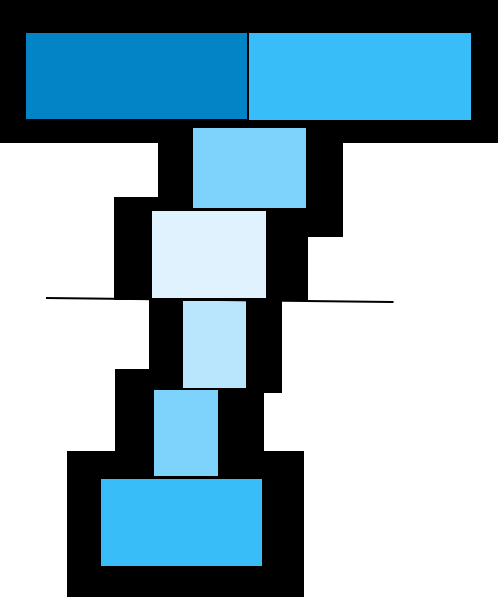
\includegraphics[width=0.25\linewidth]{Images/TemporaLogo_big.png}
    \caption{Logo Tempora}
    \label{fig:logo}
\end{figure}